\documentclass[a4paper,11pt]{article}

\usepackage[english,listings,algo]{tcs}

% Cover %
\def \ttprofname{Margaret Armstrong} % teachers name
\def \ttabrv{MP17} % abbreviation of names class
\def \ttabrvxt{ATHENS} % period
\def \mytitle{Report Project Finance - Non Recourse Finance} % Big title
\def \mysubtitle{Analysing Business Plans for telecom Projects} % subtitle
\def \ttauthi{Tiago Chedraoui Silva} % author's name
\def \ttxti{} % Extra text right side of name
\def \ttdate{November 18, 2011} % date

%\spc{2} % double spacing

\usepackage{fancyhdr}

\lhead{\footnotesize \parbox{11cm}{Tiago Chedraoui Silva} }
%\rfoot{\footnotesize Tiago Chedraoui Silva}


\begin{document}
\titleTMB 
\newpage
%\tableofcontents
%\newpage

\pagestyle{fancy}

\section{Analyzing Business Plans for telecom Projects}
\subsection{Telecom Project Business Model}

Nowadays, a great  number of different communication technologies have an important role in a Telecom projects. These technologies are mainly defined by two characteristics, which are data rate and mobility.
To achieve more data per time,in other words "high data rates", fixed technology, like optical  fiber, are used. That is possible because the environment of a optical fiber does not receive external perturbation. However, being a fixed technology it doesn't provides mobility to the user.
On the other hand, technologies which  privilege the mobility, like the GSM,  can't provides  a high data rate, because the environment it works receives external perturbation.

The figure \ref{fig:tel_tech} shows the characteristics of some technologies.

\begin{figure}[h!]
\begin{centering}
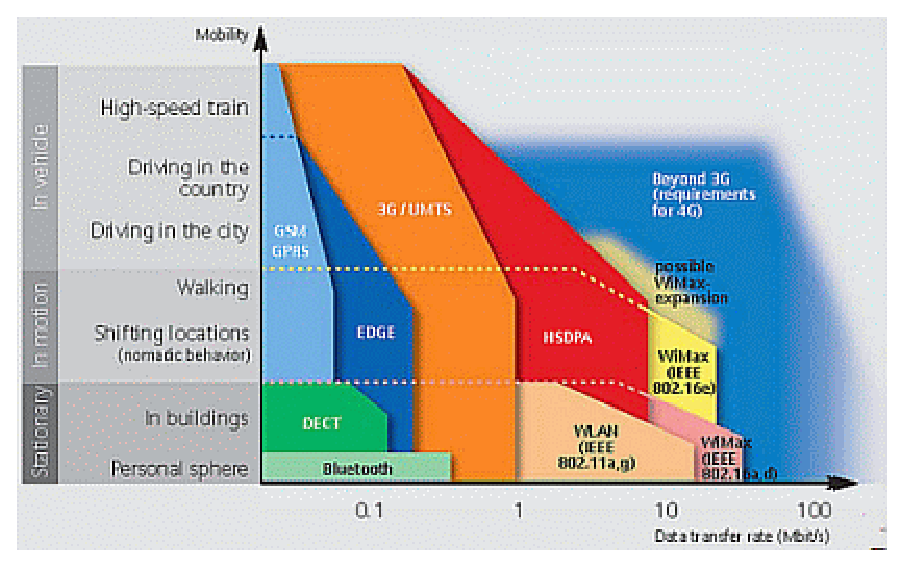
\includegraphics[scale=0.8]{szenbild_1224832}
\par\end{centering}
\caption{Characteristics of Telecom technologies \protect\footnotemark}
\label{fig:tel_tech}
\end{figure}
\footnotetext{Source:\href{http://www.siemens.com/innovation/en/publikationen/publications_pof/pof_fall_2004/always-on_articles/trends.htm}{Siemens}}



Having these different technologies to implement a telecom project, it is first needed to choose which one is the  most properly. For this, some simple questions should be made.

\begin{description}
\item[What is the business model?]  You should specify the organization from a
  high level of perspective (its purpose, offerings, strategies, infrastructure, etc.).
\item[Technology or service driven?] Which one will be offered? Should I offer both?
\item[Is  the ecosystem  ready?] Where  I'm  going to  offer my  product? Is  it
  possible to offer this product? Does the environment offer a necessary
    infrastructure?
\end{description}

Revenues had  a slightly increasing  if compared with  past years, on  the other
hand, the global traffic  has tripled in three years and it  is expected that it
will increase more in the next  years. So, today, revenues does not increases as
fast as the traffic.

Analyzing the  data, revenues  had a slightly  increasing if compared  with past
years, on the other  hand, the global traffic has tripled in  three years and it
is expected  that it will increase more  in the next years.  So, today, revenues
does not increases as fast as the traffic.Other interesting data: voice, although being a small part of the traffic
(20\% of total traffic), is the most profitable (80\% of revenues)

If a company will offer the infrastructure for telecommunication, some challenges
like finding the right mix of services and understand the market drivers will be
needed, because a company should offer only what costumer wants, and some times,
they want  both mobility  and high data  rates which  implies in a  difficult to
choose technologies and probably a high cost of implementation.

Although some companies are concerned about infrastructures (which have high costs), others are concerned
about offering a service using  an infrastructure created by other companies, so
they have low cost to offer its product.
For example,  Google, Facebook and Twitter, offer a service based on  a  software that  is connected  to
Internet which  uses   physical  links   implemented  by   telephone
companies. It is  remarkable that these companies don't  have infrastructure
costs, then, we can say that they are ``eating food of other''.



\subsection{Business Planning in Telecom Projects}
Business Planning in Telecom Projects have five phases:

\begin{description}
\item[Market] In this phase it is needed a demographic and economic study to 
  answer some questions like: What is the  country population and growth  rate? What is  population's capacity of
  spending money?  Which will probably be  the ARPU (Average  Revenue Per User)?
  And  how much  SIM cards  each  person would  have?\footnote{Depending in  the
    country some devices like GPS, PC and dual-chip mobile phones uses other SIM card, so a
    person would buy more than one SIM card} 
\begin{description}
\item[Marketing External factors] {\color{blue}1.  Country and market environment:} Demand,
  competitors, possibility  and level of  portability (change of  operator), How
  much does it cost  to construct  an infrastructure  in the  country (for  example to
  construct and maintain an antenna in Africa costs a lot, because of the cost of energy)etc. {\color{blue}2.  License and
  regulatory framework:} what is the best technology, what is the spectrum I'll
  be able  to work with, is it  acceptable for the service  offered? Which areas
  will be  covered? Will I cover only  overpopulated areas or I'll  offer a full
  mobility even if  I have a less crowded area? etc.  {\color{blue}3. Consumer behavior:} how
  much my  consumer will  consume? How the  most part  of the payments  are done
  (prepaid or postpaid)? etc.

\item[Marketing Internal factors] When my  network will be working? Which are my
  marketing strategies? How much I have to finance the structure?  etc. One 
  great idea is to compare market studies about one country, with another study
  done by competitors about a similar country.

\end{description}

\item[Revenues] In  this phase we  will estimate our  ARPU based in:  price per
  service,  price  per bundled  package,  price  trends  and forecasted  revenue
  mix.  After  we estimate  average  number of  user  based  in: traffic,  usage
  patterns, addressable market etc; So with {\color{red}ARPU} and an {\color{red}average number of users},
  multiplying both value will give us the {\color{red}service revenue.}

\item[Capital expenses]  In this phase we  will estimate our  expenses, in other
  words, we  will sum all  costs. Firstly we  have {\color{purple}infrastructure
    costs},  which is the  infrastructure need  to be  be built  in order  to be
  possible  to offer  my  service/product.  Secondly, we  have  cost related  to
  costumers  and   Site,  for   example,  instalation  cost,   customer  premise
  equipement. Thirdly, we  have License Fee, which are tax needed  to be paid in
  order use  a spectrum  for data transmission.  Moreover, we should  consider a
  replacement cost, which  is the cost if I lose some  costumer. Indeed, a great
  difficult of telecommunication  business is not only to  retrieve clients, but
  also to mantain them for a long time.
 % keep costumers -> traffic risks
\item[Operational  expenses] In  this  phase we  will  estimate the  operational
  costs, which are composed by two different types of costs: variable costs, and
  fixed costs;
  Variable  cost  depends  on  external  factor, for  example,  Roaming  Charges
  dependes on the  operator that did the service for  your company abroad, other
  examples are  Marketing cost, that may  be bigger or smaller  depending in how
  much consumers we already have;
  Differently, fixed costs, which are not dependable of external factor, for example, Office costs, spectrum license,
  Administrative  personnel,  they  can  be  meseured  without  having  external
  influence as long as they have a fixed price.


\item[Free cash flow] Finally, based  in Revenues and expenses, and some metrics
  we will make a cash flow analysis.
\end{description}

\subsection{Business Plan Key Output}

In this phase, given financial statements, and using Key metrics, we can analyze
both loan payment (Payback)  and FCF (free cash flow).
Two main objective are: have a  FCF positive, that means, income is greater  than expenses; and pay your debt, which can be viewed by positive accumulated free cash flow.


But, are my expectations reasonable? Depending on the project is will be;
For the  Payback Year, if it  is a GSM project  in six to eight  years, debt
should be payed, if its an optical network, it will take more than ten years.
For a  positive FCF, if  it is a  GSM project in three  to four years  it should
happen, if an optical network from seven to nine years should be reasonable;

\subsection{Funding Plan and Milestones}


\subsection{Sensitivity Analysis}
In this part, firstly, we should review our numbers, for that we could compare what we
got we existing ones (benchmark). Secondly, every risk should be take in account,
because they  can change the sceneraio,  for example, if the  construction of an
antenna  is  delayed,  how  does  it  will  impact in  the  project?  And  if  I
miscalculated ARPU? What if inflation rises and local currency depreciates? Does
my business plan handles with that?
What is the worst scenatio? How my bussiness plan will work in that scenario?

\end{document}
